\subsection{Spielwelt und Kamera}

Die Spielwelt (Illustration s. \figref{fig:hud}) besteht aus einem System von
Blutbahnen, dem Blutkreislauf, in dem sich die Zellen des Spielers und die
gegnerischen Viren und Bakterien aufhalten.

Die Kamera zeigt stets einen Ausschnitt des Blutkreislaufs, wobei die Größe
des dargestellten Ausschnitts und seine Position vom Spieler wählbar sind.

Gegnerische Einheiten und rote Blutkörperchen sind für den Spieler nur
sichtbar, sofern sie sich im Sichtkreis einer seiner Einheiten befinden. Die
Teile der Spielwelt, die nicht im Sichtkreis einer solchen Einheit liegen,
werden abgedunkelt dargestellt (\enquote*{Fog of War}).

\begin{figure}
  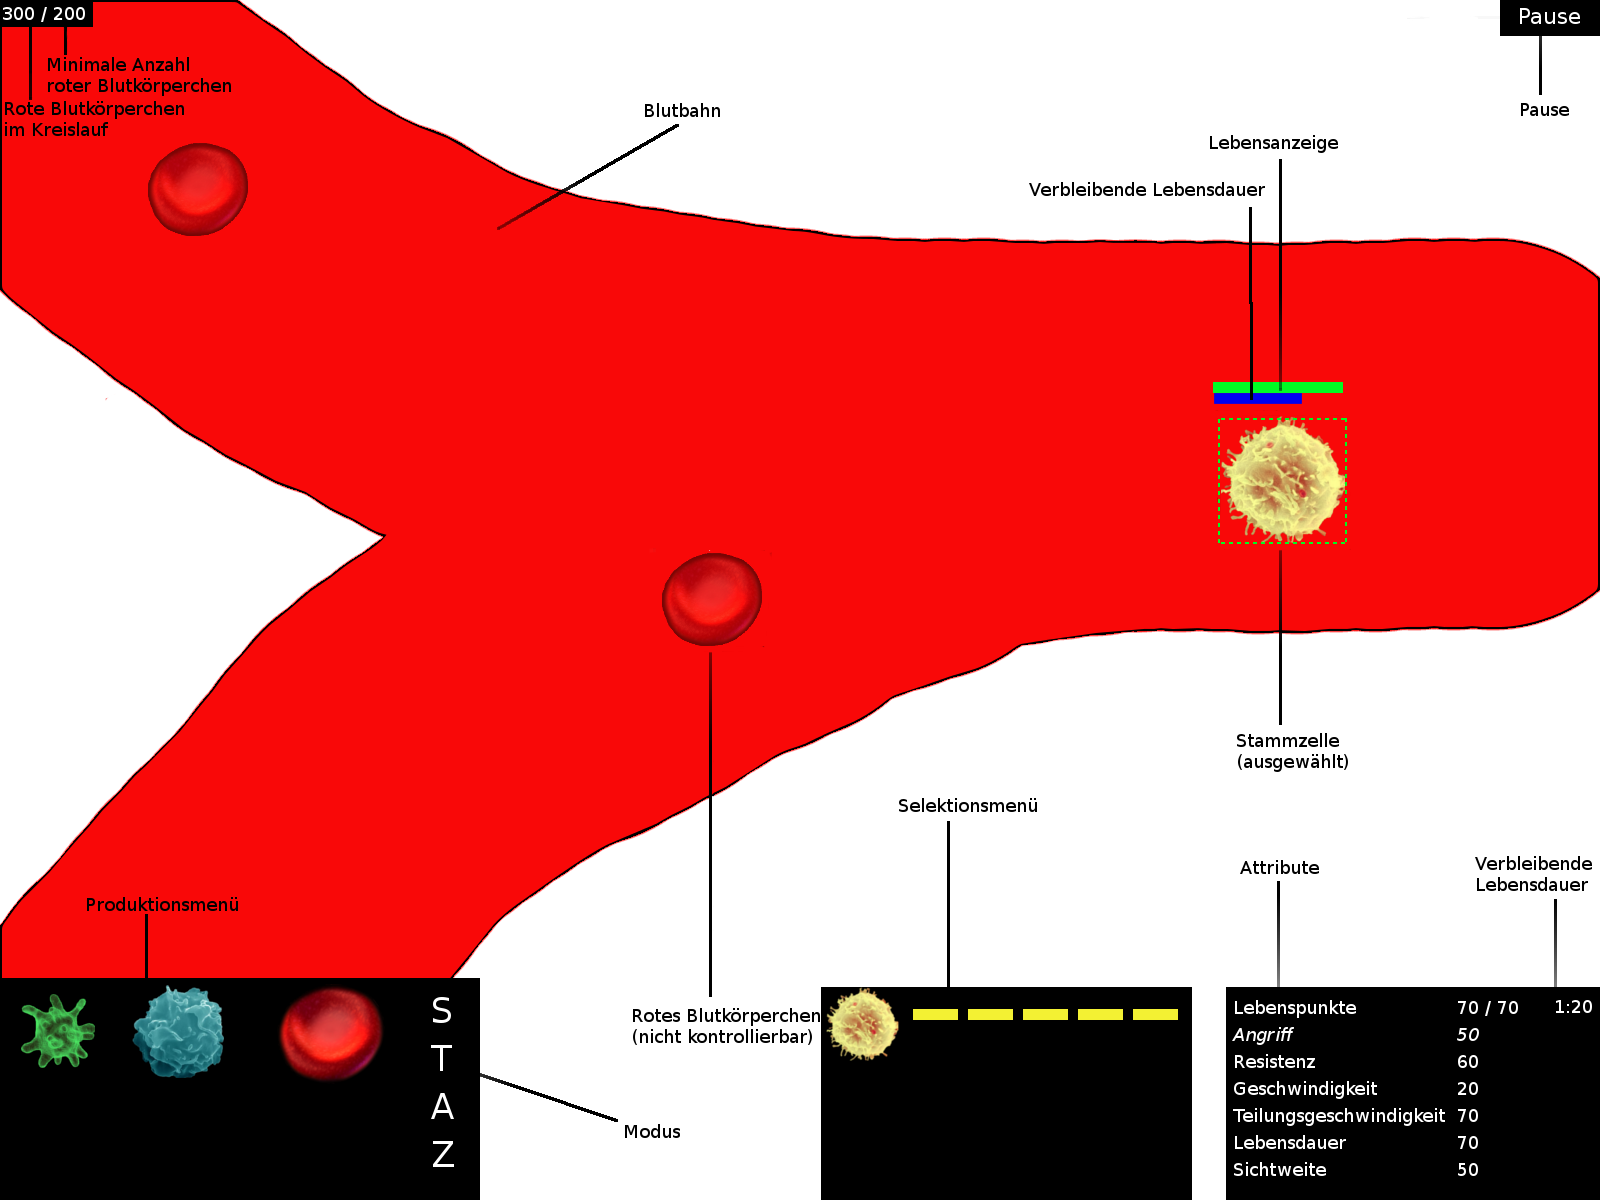
\includegraphics[width=\textwidth]{img_ui/hud}
  \caption{Spielwelt und Heads Up Display (Konzept)}
  \label{fig:hud}
\end{figure}

\subsection{Kontrollschema}

\name{} wird vorwiegend mit der Maus gesteuert: Alle Aktionen können allein mit
der Maus vorgenommen werden, aber für manche sind auch Tastenkombinationen
definiert. Im folgenden Überblick über das Kontrollschema ist jeweils die
Standardtastenbelegung angegeben.

Das Produktionsmenü, die Modusauswahl und der Link zum Pausemenü sind
Elemente des Heads Up Displays, die in \figref{fig:hud} illustriert sind.

\newcommand*{\shortcut}[1]{\textbf{#1}}

\begin{description}
  \item[Cursorbewegung] Wird der Cursor an den Rand des Spielfensters
    geführt, so wird die Karte in die entsprechende Richtung bewegt, sofern
    sie in dieser Richtung nicht bereits den Rand der Karte erreicht hat.
  \item[Mausrad] Ein Drehen des Mausrads nach vorn zoomt in das Spiel herein;
    ein Drehen nach hinten aus dem Spiel heraus.
  \item[Linke Maustaste] Ein Klick auf eine auswählbare Einheit wählt diese
    aus. Durch Klicken und Halten kann ein Rechteck aufgezogen werden, mit
    dem alle auswählbaren Einheiten in einem Bereich ausgewählt werden.
  \item[Rechte Maustaste]
    Die Belegung der rechten Maustaste variiert abhängig von der ausgewählten
    Einheit und dem Ziel des Klicks.
    \begin{itemize}
      \item Ausgewählte bewegbare Einheit, Klick auf den Boden: Die ausgewählte
        Einheit bewegt sich zum angegebenen Punkt oder, wenn das nicht
        möglich ist, zu einem möglichst nahen erreichbaren Punkt.
      \item Ausgewählte angreifende Einheit, Klick auf eine gegnerische Einheit:
        Sofern die ausgewählte Einheit die gegnerische Einheit angreifen kann,
        bewegt jene sich zu dieser und attackiert sie.
      \item Ausgewählte antigenverarbeitende Einheit, Klick auf Riesenfresszelle:
        Sofern die Riesenfresszelle ein Antigen aufgenommen hat, bewegt sich
        die ausgewählte Einheit zu ihr und übernimmt das Antigen.
      \item Ausgewählte Riesenfresszelle mit Antigen, Klick auf
        antigenverarbeitende Zelle: Die Riesenfresszelle bewegt sich zur
        angeklickten Einheit und übergibt ihr das Antigen.
    \end{itemize}
  \item[Überblick] (\shortcut{Leertaste}) Verändert den Kameraausschnitt so,
    dass die Spielwelt vollständig sichtbar ist.
  \item[Produktionsmenü] Produziert bei ausgewählter Stammzelle eine
    B-Zelle (\shortcut{B}), T-Zelle (\shortcut{T}), Riesenfresszelle
    (\shortcut{F}) oder ein Rotes Blutkörperchen (\shortcut{R}). Bei
    ausgewählter B-Zelle kann ein Antikörper (\shortcut{A}) produziert werden.
    Siehe auch \secref{sec:zellen}.
  \item[Modusauswahl] Wählt bei ausgewählter eigener Einheit einen der vier
    Zellmodi (siehe \secref{sec:modi}) aus: Stellung halten (\shortcut{S}),
    Treiben lassen (\shortcut{L}), Angriff (\shortcut{P}) oder Zellteilung
    (\shortcut{Z}).
  \item[Pause] Pausiert das Spiel (\shortcut{Esc}).
\end{description}

\subsection{Heads Up Display}

Außer den im letzten Abschnitt erwähnten interaktiven Elementen des HUD
(\figref{fig:hud}) enthält dieses noch die folgenden informativen Elemente:

\begin{description}
  \item[Zähler für Rote Blutkörperchen:] Zeigt die aktuelle Anzahl Roter
    Blutkörperchen im Blutkreislauf und die Minimalanzahl, bei deren
    Unterschreitung das Spiel verloren ist.
  \item[Lebensanzeigen:] Grafische Repräsentation der aktuellen Lebenspunkte
    jeder ausgewählten Einheit.
  \item[Attributanzeige:] Aktuelle Werte der Eigenschaften
    (s.~\tabref{tab:eigenschaften}) der ausgewählten Einheit.
  \item[Verbleibende Lebensdauer:] Anzeige der verbleibenden Zeit, nach der die
    ausgewählte Einheit \enquote*{natürlich} stirbt.
  \item[Selektionsmenü:] Liste aller selektierten Einheiten mit einer
    Übersicht über ihre Attributwerte.
\end{description}

\subsection{Menüstruktur}

\subsubsection{Hauptmenü}
\label{menu:hauptmenu}

\begin{description}
  \item[Neues Spiel] (\ref{menu:neues_spiel})
  \item[Laden] (\ref{menu:laden})
  \item[Optionen] (\ref{menu:optionen})
  \item[Achievements] (\ref{menu:achievements})
  \item[Ende] Beendet das Programm.
\end{description}

\subsubsection{Pause}
\label{menu:pause}

\begin{description}
  \item[Fortsetzen] Kehrt zum Spiel zurück.
  \item[Speichern] (\ref{menu:speichern})
  \item[Laden] (\ref{menu:laden})
  \item[Optionen] (\ref{menu:optionen})
  \item[Statistiken] (\ref{menu:statistiken})
  \item[Achievements] (\ref{menu:achievements})
  \item[Hauptmenü] Beendet das aktuelle Spiel, ohne zu speichern, und kehrt
    zum Hauptmenü zurück.
  \item[Ende] Beendet das Programm.
\end{description}

\subsubsection{Neues Spiel}
\label{menu:neues_spiel}

Auswahl der Karte und des Schwierigkeitsgrads für ein neues Spiel.

Der Schwierigkeitsgrad kann die Werte Leicht/Mittel/Schwer annehmen. Ein
leichterer Schwierigkeitsgrad erhöht die Werte einiger Einheiten des
Spielers und senkt die einiger Einheiten der KI. Er modifiziert \textbf{optional}
auch das Verhalten der KI, wobei ein leichterer Schwierigkeitsgrad dazu führt,
dass die KI mehr taktische Fehler begeht.

\subsubsection{Speichern}
\label{menu:speichern}

Zeigt eine Liste mit vorhandenen Spielständen. Das aktuelle Spiel kann entweder
einen dieser Spielstände überschreiben oder als neuer Spielstand gespeichert
werden. Für Spielstände können Namen vergeben werden, außerdem sind sie mit
einer eindeutigen Nummer gekennzeichnet.

\subsubsection{Laden}
\label{menu:laden}

Zeigt eine Liste mit vorhandenen Spielständen, von denen einer ausgewählt
werden kann.

\subsubsection{Optionen}
\label{menu:optionen}

Ermöglicht die Anpassung der folgenden Optionen (ggf. mit eigenen Untermenüs):

\begin{description}
  \item[Kamerageschwindigkeit:] 0,5x bis 2x. Multipliziert die Geschwindigkeit
    der Kamerabewegung bei Veränderung des Kameraausschnitts mit dem
    entsprechenden Faktor.
  \item[Auflösung:] Modifiziert die Auflösung der grafischen Darstellung des
    Spiels. Der Spieler kann jede Auflösung wählen, die sein Anzeigegerät
    unterstützt. Die Spielbarkeit des Spiels wird allerdings nur für
    Auflösungen zwischen 1024x798 und 1920x1080 Pixeln garantiert.
  \item[Vollbild:] Stellt das Spiel im Vollbildmodus dar. Ist diese Option
    nicht ausgewählt, so wird das Spiel im Fenstermodus dargestellt.
  \item[Audio:] Modifiziert die Lautstärke der Spielsounds. Separate Optionen
    für Master-, Musik- und Effektlautstärke.
  \item[Tastenbelegung:] Assoziiert Aktionen mit Tasten.
\end{description}

\subsubsection{Statistiken}
\label{menu:statistiken}

Zeigt Statistiken (s.~\secref{sec:statistiken}) für das gerade laufende Spiel
an.

\subsubsection{Achievements}
\label{menu:achievements}

Zeigt die bislang über alle Spiele errungenen Achievements
(s.~\secref{sec:achievements}) an.
